\chapter{Gamma Distribution ($X \sim G(\alpha, \beta)/ G(k,\theta)$) \cite{ism-1,wiki/Gamma_distribution}}\label{Gamma Distribution}

\begin{table}[H]
    \begin{minipage}{0.49\linewidth}
        \begin{figure}[H]
            \centering
            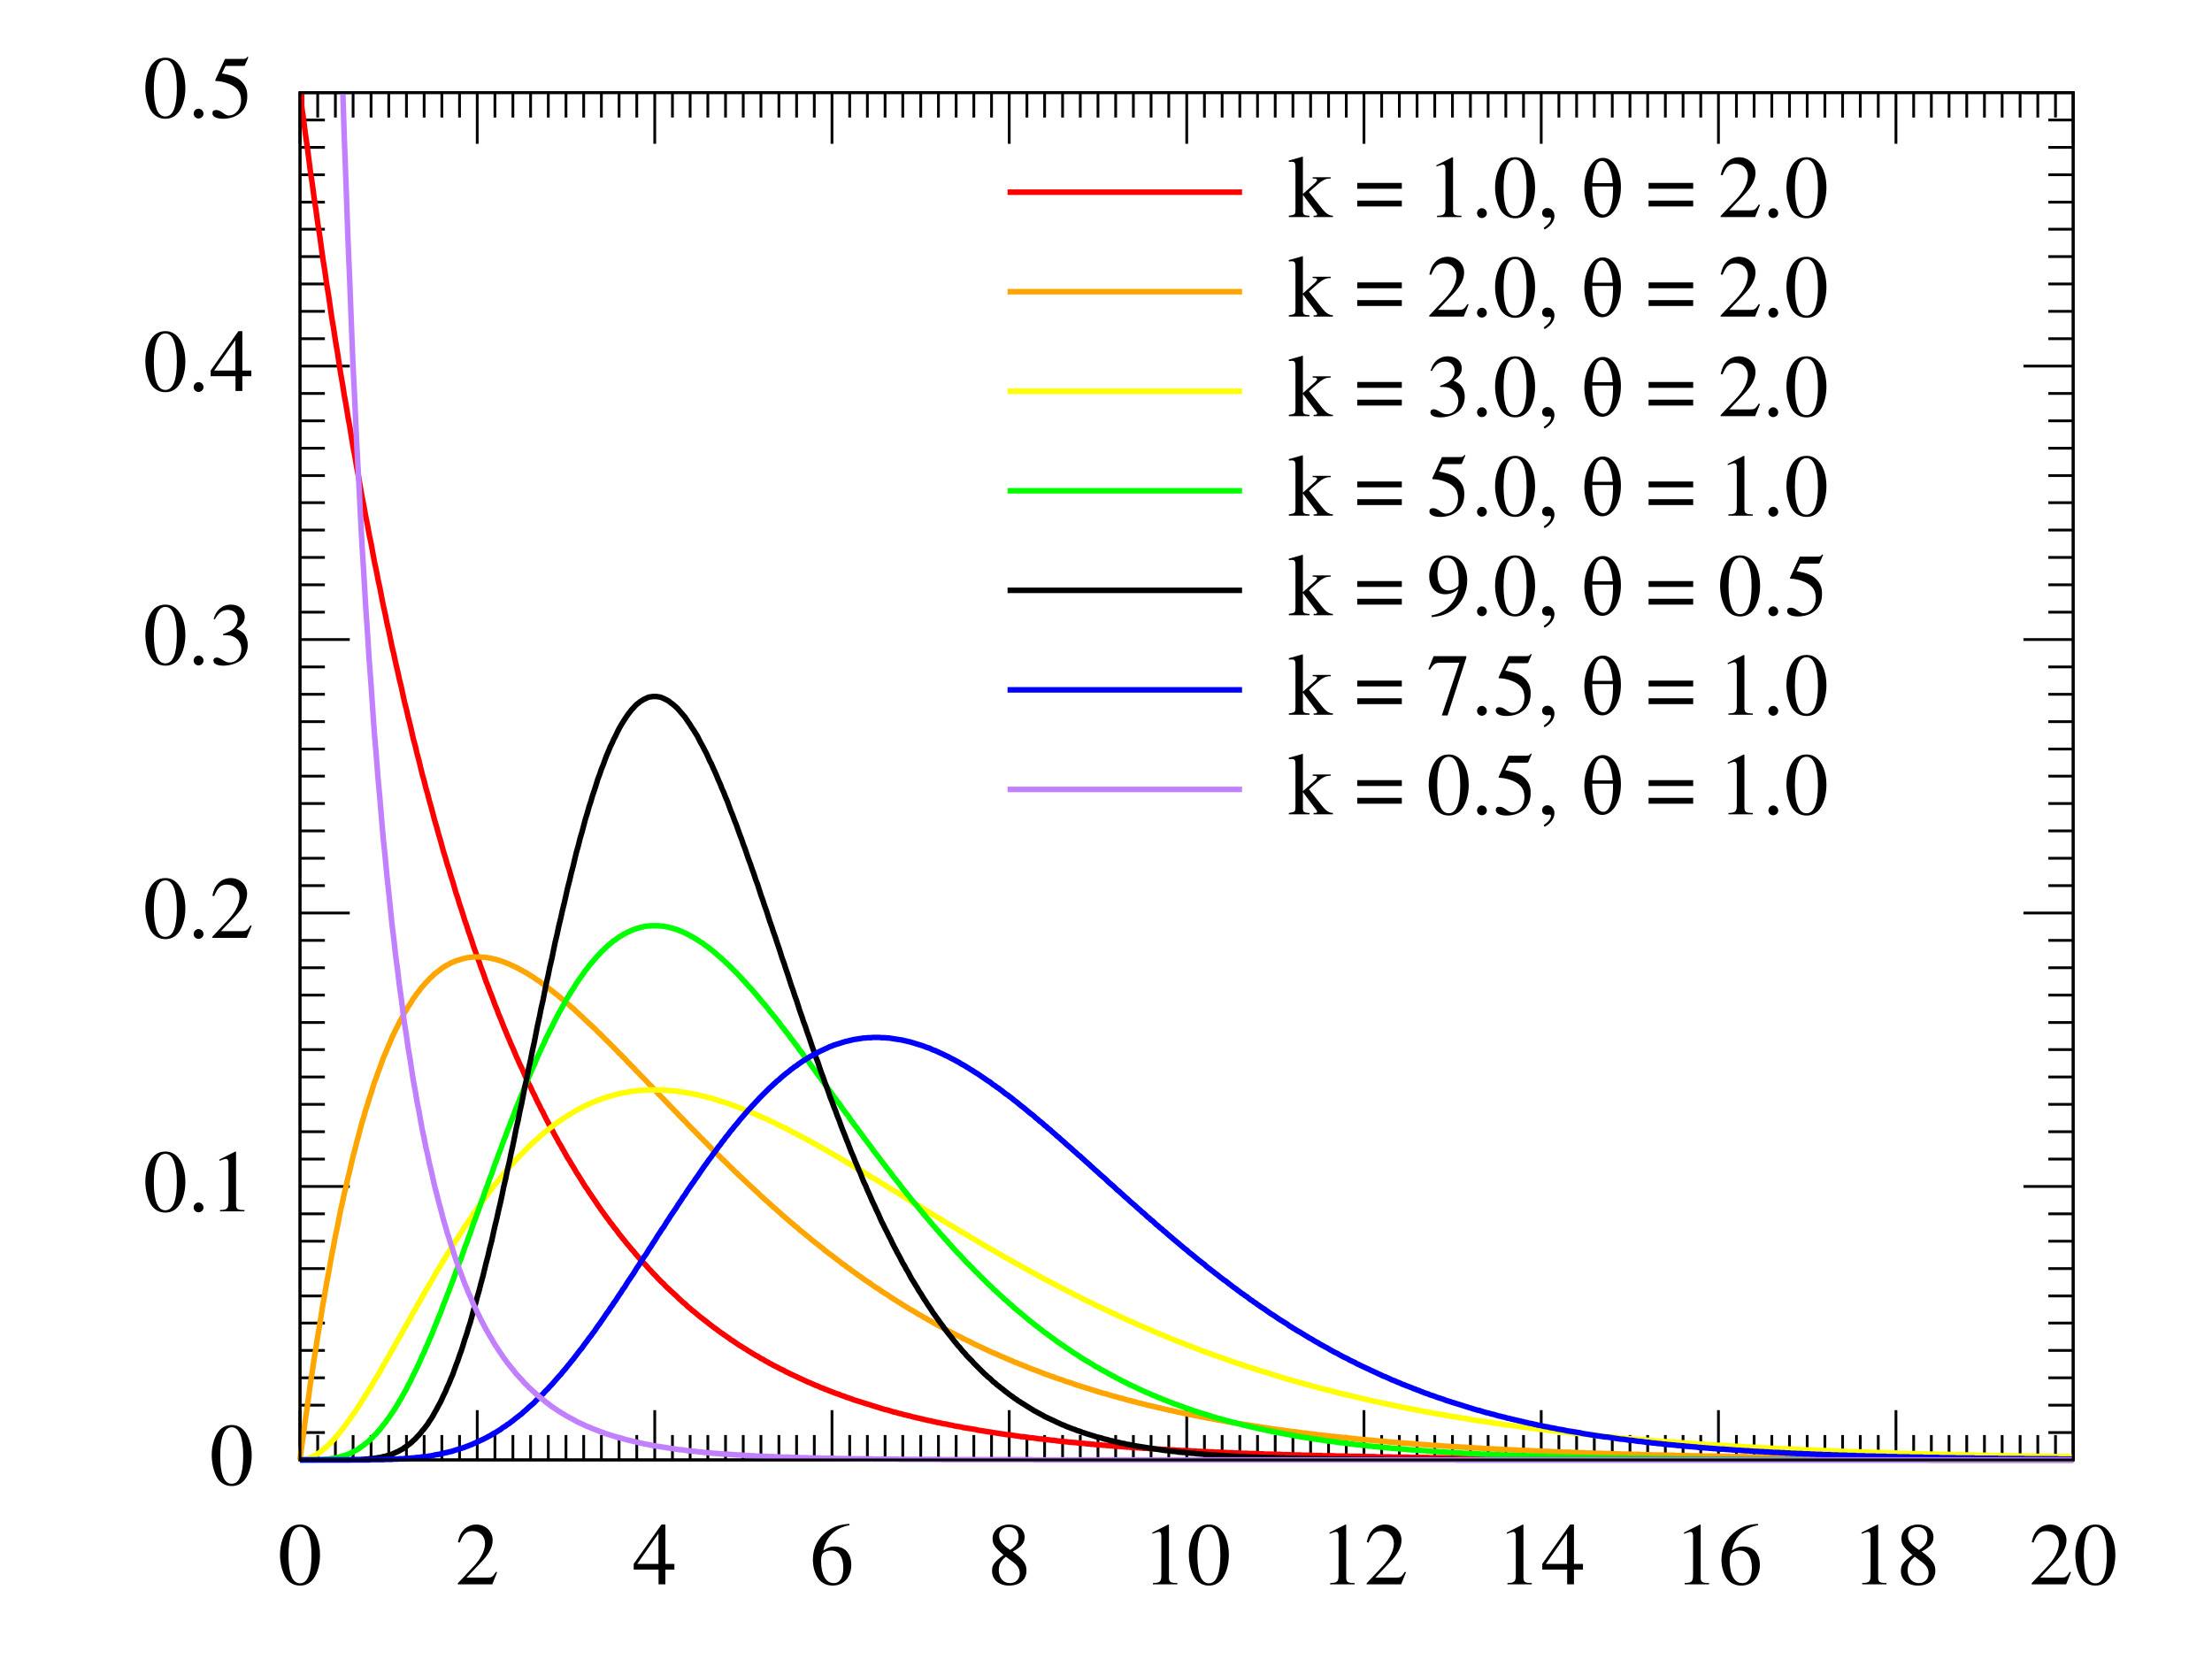
\includegraphics[width=\linewidth, height=4cm, keepaspectratio]{Pictures/distributions/Gamma_distribution_pdf.jpg}
            \caption{Gamma distribution: PDF}
        \end{figure}
    \end{minipage}
    \hfill
    \begin{minipage}{0.49\linewidth}
        \begin{figure}[H]
            \centering
            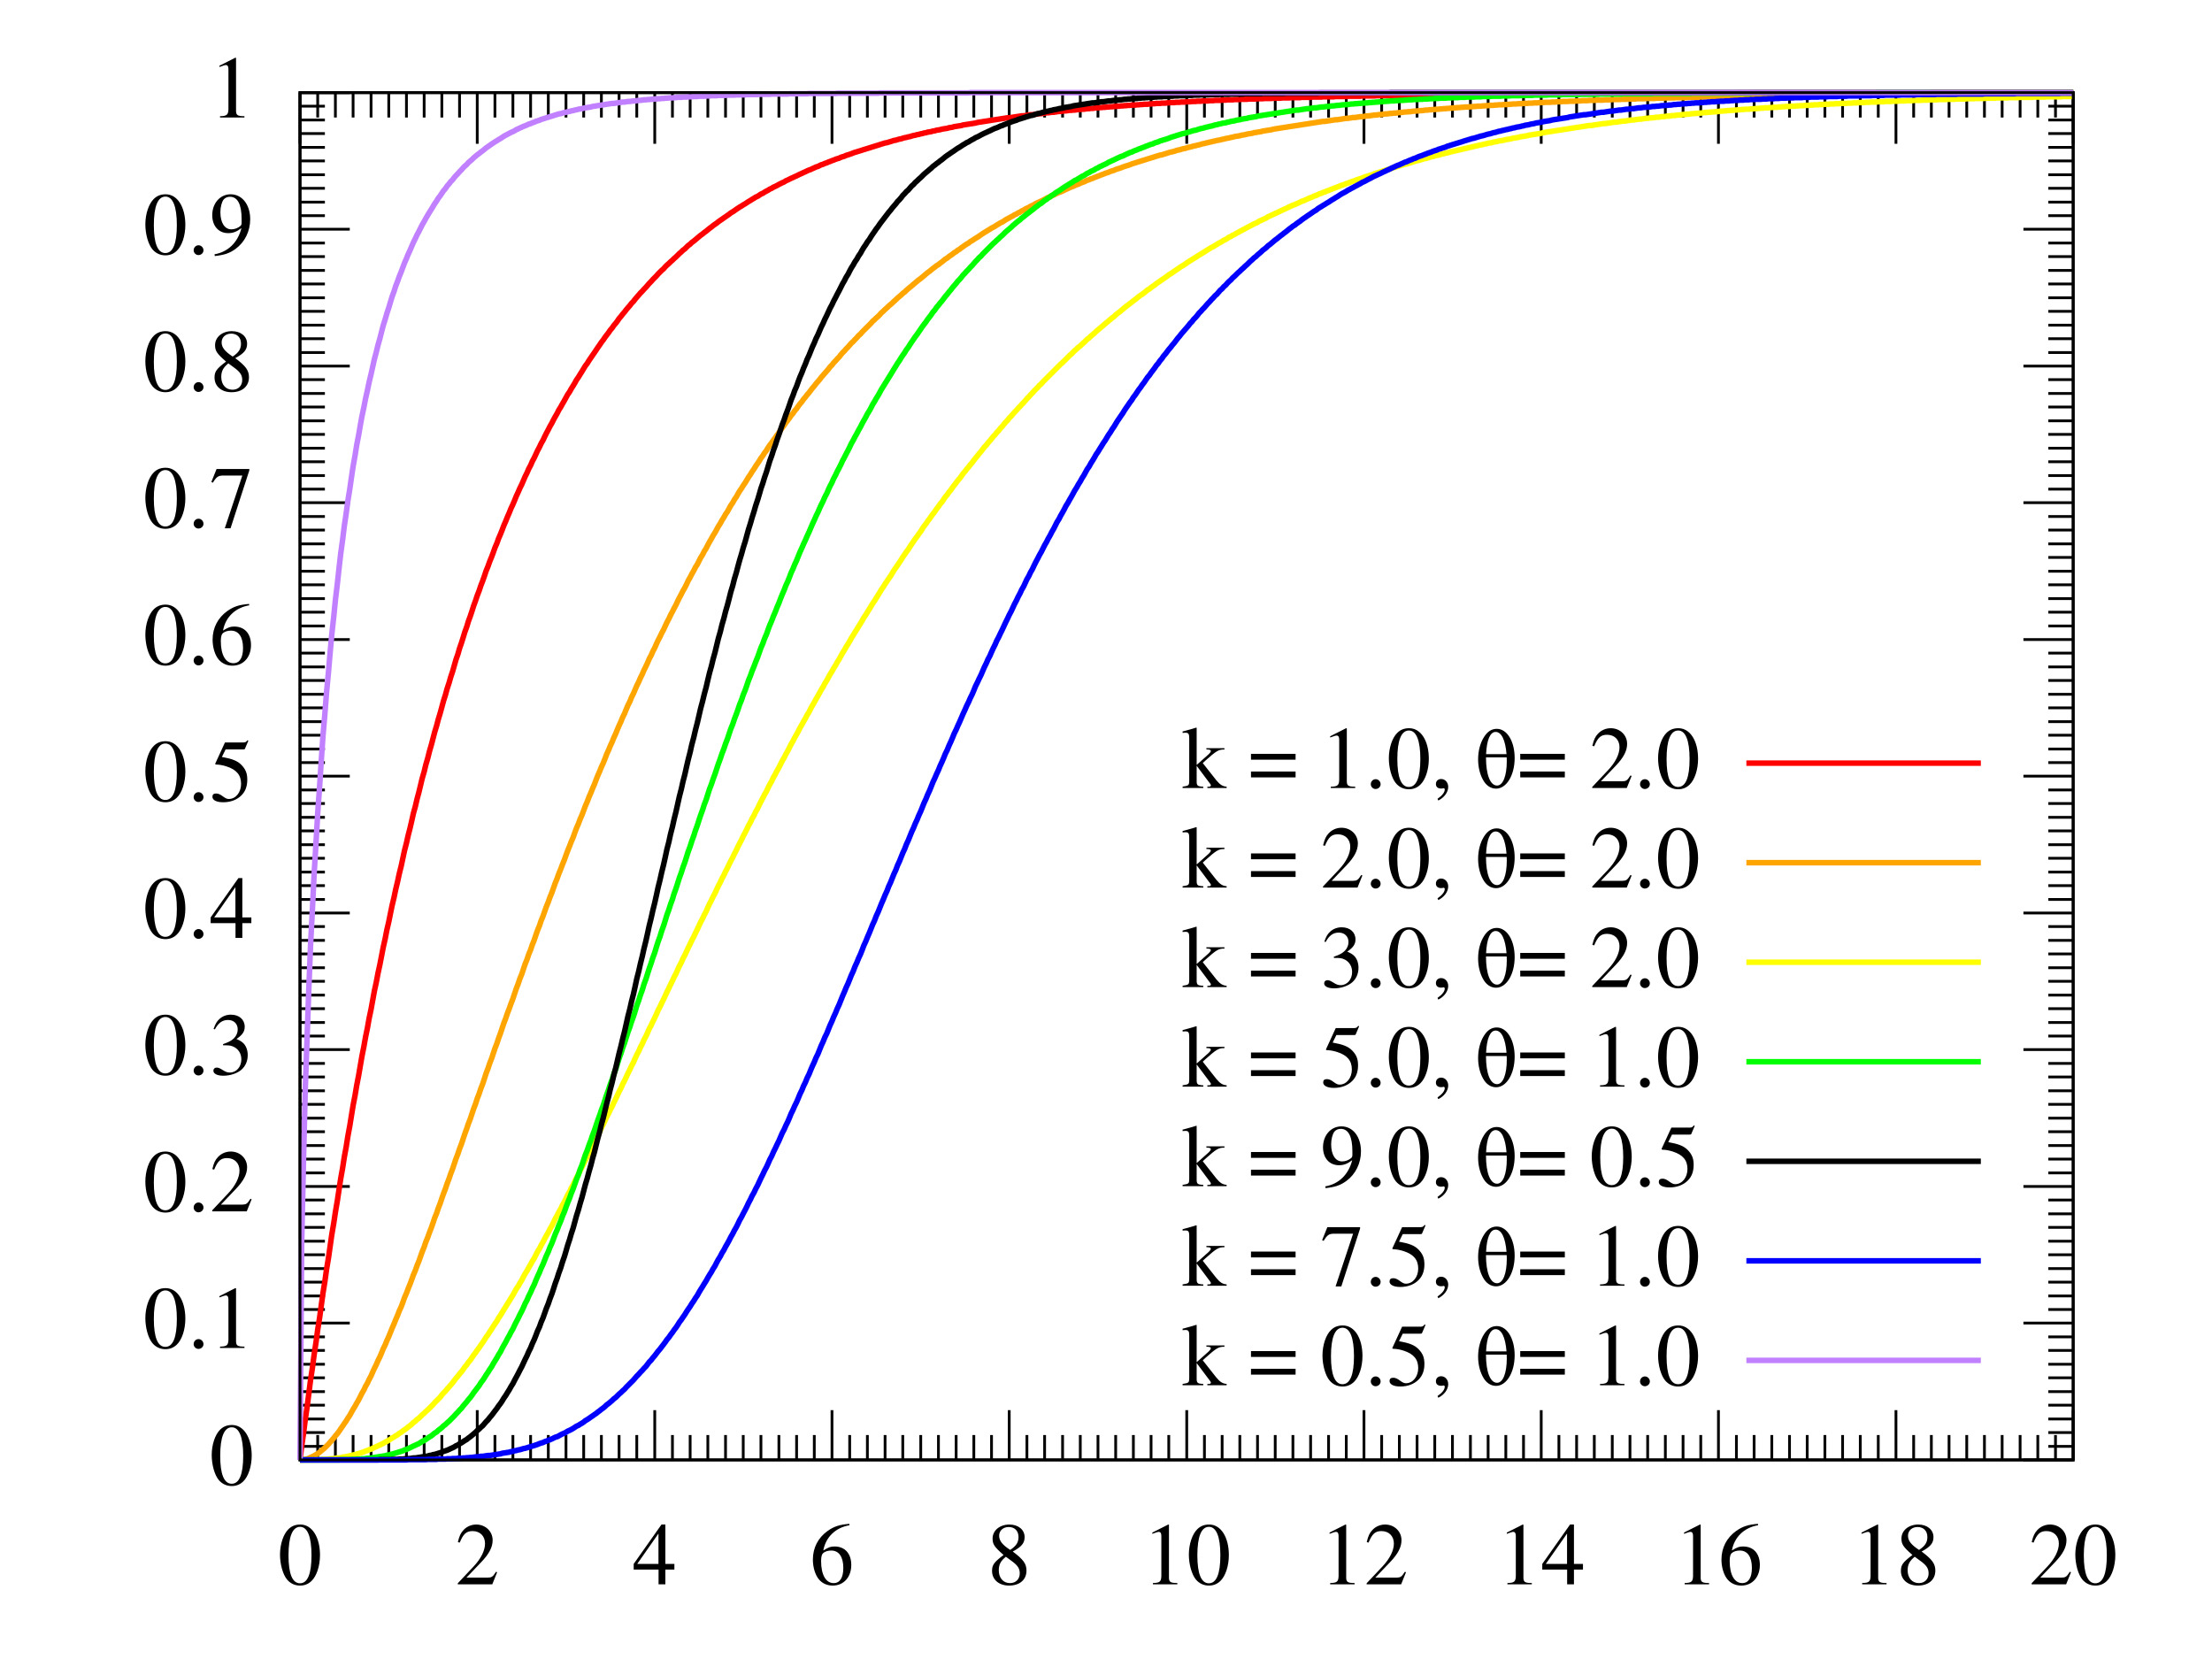
\includegraphics[width=\linewidth, height=4cm, keepaspectratio]{Pictures/distributions/Gamma_distribution_cdf.jpg}
            \caption{Gamma distribution: CDF}
        \end{figure}
    \end{minipage}
\end{table}

\begin{customTableWrapper}{2}
\begin{longtable}{|m{3cm}|p{5.5cm}|p{5.5cm}|}
    \hline
    \customTableHeaderColor
    \multicolumn{3}{|c|}{\textbf{Gamma Distribution - Info} \cite{wiki/Exponential_distribution}} \\ \hline
    & $G(k,\theta)$ & $G(\alpha, \beta)$ \\
    \hline\endfirsthead

    \hline
    \customTableHeaderColor
    \multicolumn{3}{|c|}{\textbf{Gamma Distribution - Info - contd.} \cite{wiki/Exponential_distribution}} \\ \hline
    & $G(k,\theta)$ & $G(\alpha, \beta)$ \\
    \hline\endhead
    
    \hline\endfoot
    \hline\endlastfoot

    \textbf{Statistical parameters} & 
    \tableenumerate{
        \item $k > 0$ shape
        \item $\theta > 0$ scale
    } &
    \tableenumerate{
        \item $\alpha > 0$ shape
        \item $\beta > 0$ rate
    }
    \\ \hline
    
    \textbf{Support} &
    \multicolumn{2}{|c|}{${ x\in (0,\infty )}$}
    \\ \hline

    \textbf{Probability Density Function (PDF)} & 
    ${ f(x)={\dfrac {1}{\Gamma (k)\theta ^{k}}}x^{k-1}e^{-x/\theta }}$ &
    ${ f(x)={\dfrac {\beta ^{\alpha }}{\Gamma (\alpha )}}x^{\alpha -1}e^{-\beta x}}$
    \\[1ex] \hline
    
    \textbf{Cumulative distribution function (CDF)} & 
    ${ F(x)={\dfrac {1}{\Gamma (k)}}\gamma \left(k,{\dfrac {x}{\theta }}\right)}$ &
    ${ F(x)={\dfrac {1}{\Gamma (\alpha )}}\gamma (\alpha ,\beta x)}$
    \\ \hline

    \textbf{Mean} & 
    ${ k\theta }$ &
    ${ {\dfrac {\alpha }{\beta }}}$
    \\[1ex] \hline

    \textbf{Median} & 
    \multicolumn{2}{|c|}{No simple closed form}
    \\[1ex] \hline

    \textbf{Mode} & 
    \tableenumerate{
        \item ${ (k-1)\theta {\text{ for }}k\geq 1}$ 
        \item ${ 0{\text{ for }}k<1}$
    } &
    ${ {\dfrac {\alpha -1}{\beta }}{\text{ for }}\alpha \geq 1{\text{, }}0{\text{ for }}\alpha <1}$
    \\ \hline

    \textbf{Variance} &
    ${ k\theta ^{2}}$ &
    ${ {\dfrac {\alpha }{\beta ^{2}}}}$
    \\[1ex] \hline

    \textbf{Skewness} &
    ${ {\dfrac {2}{\sqrt {k}}}}$&
    ${ {\dfrac {2}{\sqrt {\alpha }}}}$
    \\[1ex] \hline

    \textbf{Excess kurtosis} &
    ${ {\dfrac {6}{k}}}$&
    ${ {\dfrac {6}{\alpha }}}$
    \\[1ex] \hline

    \textbf{Entropy} &
    ${ {\begin{aligned}k&+\ln \theta +\ln \Gamma (k)\\&+(1-k)\psi (k)\end{aligned}}}$&
    ${ {\begin{aligned}\alpha &-\ln \beta +\ln \Gamma (\alpha )\\&+(1-\alpha )\psi (\alpha )\end{aligned}}}$
    \\[1ex] \hline

    \textbf{Moment-generating function (MGF)} &
    ${ (1-\theta t)^{-k}{\text{ for }}t<{\dfrac {1}{\theta }}}$&
    ${ \left(1-{\dfrac {t}{\beta }}\right)^{-\alpha }{\text{ for }}t<\beta }$
    \\[1ex] \hline

    \textbf{Characteristic function (CF)} &
    ${ (1-\theta it)^{-k}}$&
    ${ \left(1-{\dfrac {it}{\beta }}\right)^{-\alpha }}$
    \\[1ex] \hline

    \textbf{Fisher information} &
    ${ I(k,\theta )={\begin{pmatrix}\psi ^{(1)}(k)&\theta ^{-1}\\\theta ^{-1}&k\theta ^{-2}\end{pmatrix}}}$&
    ${ I(\alpha ,\beta )={\begin{pmatrix}\psi ^{(1)}(\alpha )&-\beta ^{-1}\\-\beta ^{-1}&\alpha \beta ^{-2}\end{pmatrix}}}$
    \\[1ex] \hline

    \textbf{Method of moments} &
    $
        { k={\dfrac {E[X]^{2}}{V[X]}}\quad \quad }
        \quad\quad
        { \theta ={\dfrac {V[X]}{E[X]}}\quad \quad }
    $&
    $
        { \alpha ={\dfrac {E[X]^{2}}{V[X]}}}
        \quad\quad
        { \beta ={\dfrac {E[X]}{V[X]}}}
    $
    \\[1ex] \hline

\end{longtable}
\end{customTableWrapper}

\begin{enumerate}
    \item here are two equivalent parameterizations in common use:
    \begin{enumerate}
        \item With a shape parameter $k$ and a scale parameter $\theta$

        \item With a shape parameter ${ \alpha =k}$ and an inverse scale parameter ${ \beta =1/\theta }$, called a rate parameter.

    \end{enumerate}

\end{enumerate}




































